\documentclass[11pt]{scrartcl}
\usepackage{dominatrix}

% Graph Drawing Stuff
\usepackage{colortbl}
\usepackage{pgfplots}
\usepackage{tikz}
\usetikzlibrary{trees}
\usetikzlibrary{calc}
\pgfplotsset{compat=1.9}

% Tables
\usepackage{multirow}

% Strikeout
\usepackage{ulem}

% Jon's Name
\newcommand{\jon}{J\'{o}n }

% Additional Definitions
\newcommand{\og}{\ensuremath{\tilde{Y}}}

\title{Business Cycles}
\subject{ECON W3213 Spring 2014 \jon Steinsson}
\author{Linan Qiu, lq2137}

\begin{document}

\maketitle

\begin{abstract}
This set of recitation notes introduces \textbf{Business Cycles}. This is in no way a substitute for attending lectures, but just in case you dozed off or checked your boyfriend's Facebook page while \jon was working Calculus magic on the board, this set of notes may save you.
\end{abstract}

So far we've been focusing a lot on the long run. How so? We've been assuming that there is full employment, that unemployment is only at natural rate. This means that if you're out of a job, you either chose it (because you want a vacation to Disneyland in Florida) or you're just looking for another job. We simplified our lives.

But why not be a little more sadistic? After all, you won't be in this course if you weren't. Hence, now we consider short run fluctuations as well.

\section{Output Gap}

Imagine a cookie factory. It can produce 100 cookies a day. However, let's say that some workers are sick, so the factory only produces 80 cookies for today. So when it's producing 80 cookies, there's this unused capacity of 20 cookies. 

\[ 80 = 100 - 20 \]

We say that the full capacity (long run capacity) is 100 cookies with a short run fluctuation of -20 cookies. The actual output is then 80 cookies. 

If this cookie factory was an economy (and how we wish it was), we say that 

\[Y_t = \bar{Y}_t + \tilde{Y}_t \]

Where $Y_t$ is the actual output, $\bar{Y}_t$ is the long run trend, and $\tilde{Y}_t$ is the short run fluctuation (or output gap).

However, this measure isn't really meaningful. Say a cookie factory has a spare capacity of 20 cookies out of 100 cookies, while another pizza factory has a spare capacity of 50 pizzas out of 400 pizzas. We can't just measure the absolute value of the output gap. Instead, we want a definition of output gap that takes into account the capacity. So we express output gap as a percentage of the potential output.

\[ \tilde{Y}_t = \frac{Y_t - \bar{Y}_t}{\bar{Y}_t} \approx \log{\left(\frac{Y_t}{\bar{Y}_t}\right)} \]

\section{Medieval Model Expanded}

Now we can expand the medieval model that we were working with.

\subsection{Rewriting the Medieval Model}

We start with three equations

\begin{align*}
M_t \bar{V} &= P_t Y_t \\
Y_t &= \bar{A} L_t \\
\frac{P_{t+1}}{P_{t}} &= \left(\frac{L_t}{\bar{L}}\right)^\theta
\end{align*}

We can combine the last two to form

\begin{align*}
M_t \bar{V} &= P_t Y_t \\
\frac{P_{t+1}}{P_{t}} &= \left(\frac{Y_t}{\bar{Y}}\right)^\theta
\end{align*}

You can think of the first as Aggregate Demand (AD) and the second as Short Run Aggregate Supply (AS). After all, the first concerns consumption and demand (think transactions) while the second pricing decisions of suppliers.

\textbf{For AD},

\begin{align*}
\log{M_t} + \log{\bar{V}} &= \log{P_t} + \log{Y_t} \\
\log{M_t} - \log{M_{t-1}} + \log{\bar{V}} - \log{\bar{V}} &= \log{P_t} - \log{P_{t-1}}+ \log{Y_t} - \log{Y_{t-1}} \\
\Delta \log{M_t} &= \Delta \log{P_t} + \Delta \log{Y_t}
\end{align*}

Now remember that inflation $\pi_t$ is

\begin{align*}
\pi_t &= \frac{P_t - P_{t-1}}{P_{t-1}} \\
\pi_t + 1 &= \frac{P_t}{P_{t-1}} \\
\log{(\pi_t + 1)} &= \log{P_t} + \log{P_{t+1}} \\
\log{(\pi_t + 1)} &= \Delta \log{P_t} \\
\log{(\pi_t + 1)} &\approx \pi_t \\
\pi_t &\approx \Delta \log{P_t}
\end{align*}

Also, remember that output gap $\og_t$ is

\begin{align*}
\og_t &= \frac{Y_t - \bar{Y}}{\bar{Y}} \\
\og_t + 1 &= \frac{Y_t}{\bar{Y}} \\
\log{\og_t + 1} &= \log{Y_t} - \log{\bar{Y}} \\
\og_t &\approx \log{Y_t} - \log{\bar{Y}} \\
\og_t - \og_{t-1} &\approx \log{Y_t} - \log{Y_{t-1}} 
\end{align*}

This simplifies $\Delta \log{M_t}$ to

\[ \Delta \log{M_t} = \pi_t + \og_t - \og_{t-1} \]

\textbf{For SRAS}, 

\begin{align*}
\frac{P_{t}}{P_{t-1}} &= \left(\frac{Y_{t-1}}{\bar{Y}}\right)^\theta \\
\Delta \log{P_t} &= \theta \log{\left( \frac{Y_{t-1}}{\bar{V}} \right)} \\
\pi_t &= \theta \og_{t-1}
\end{align*}

So now, we have

\begin{align*}
\pi_t  &= \Delta \log{M_t} - \og_t + \og_{t-1} \\
\pi_t &= \theta \og_{t-1}
\end{align*}

Tada!

Now here's the awesome thing. The trick to this model lies in the $t$ and $t-1$.

\begin{figure}[H]
\centering
\begin{tikzpicture}
\begin{axis}[xlabel={Output Gap $\og_t$},ylabel={Inflation $\pi_t$},ymin=0,ymax=10,xmin=0,xmax=10,scale=1]
\addplot[blue, domain=0:10]
{-x+8};
\addplot[black, domain=0:10]
{5};
\end{axis}
\end{tikzpicture}
\caption{\color{blue}AD-\color{black}SRAS Diagram}
\end{figure}

Imagine that we were at full employment. By that, I mean that we're at long run equilibrium, and that $\og_t = \og_{t-1}$. Do you see what that does to our model? It makes \textbf{AD} $\pi_t = \Delta \log{M_t}$. We can mark out this special little point.

\begin{figure}[H]
\centering
\begin{tikzpicture}
\begin{axis}[xlabel={Output Gap $\og_t$},ylabel={Inflation $\pi_t$},ymin=0,ymax=10,xmin=0,xmax=10,scale=1]
\addplot[blue, domain=0:10]
{-x+8};
\addplot[black, domain=0:10]
{5};
\addplot[black, domain=0:10, dashed]
coordinates{(3,0) (3,5)};
\end{axis}
\end{tikzpicture}
\caption{\color{blue}AD-\color{black}SRAS Diagram}
\end{figure}

Now let's see what happens if the government increases $\log{M_t}$ suddenly. So let's say we were in $t=-1$. Now at $t=0$, the government expands money supply. In that case, $\pi_t$ will increase at every point of $\og_t$. This means there's an upward/outward shift of the AD.

\begin{figure}[H]
\centering
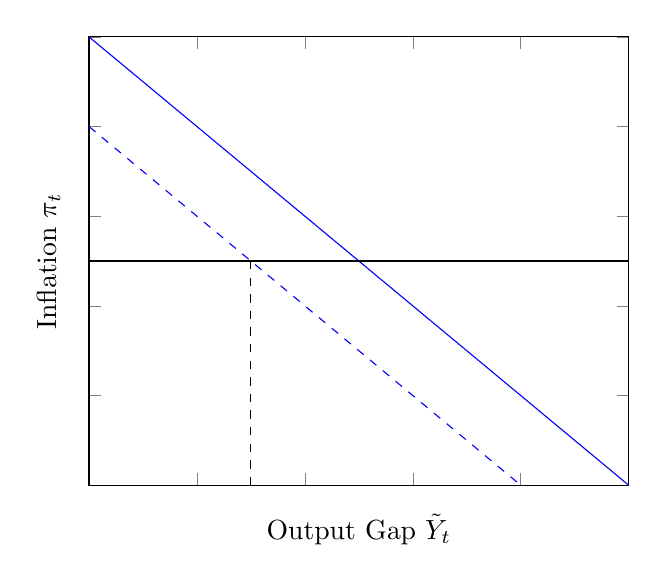
\begin{tikzpicture}
\begin{axis}[xlabel={Output Gap $\og_t$},ylabel={Inflation $\pi_t$},ymin=0,ymax=10,xmin=0,xmax=10,scale=1,yticklabels={,,},xticklabels={,,}]
\addplot[blue, domain=0:10, dashed]
{-x+8};
\addplot[blue, domain=0:10]
{-x+10};
\addplot[black, domain=0:10]
{5};
\addplot[black, domain=0:10, dashed]
coordinates{(3,0) (3,5)};
\end{axis}
\end{tikzpicture}
\caption{\color{blue}AD-\color{black}SRAS Diagram}
\end{figure}

Does the SRAS change at $t=0$? Well, no. $\pi_t = \theta \og_{t-1}$ means that it only considers the $\og$ of the previous time period, which in this case was the dotted line. Hence, it still stays like that.

However, at $t=1$, SRAS shifts up. This is because $\pi_1 = \theta \og_0$, and $\og_0$ was higher than than that of $\og_{-1}$. 

Hence, we have

\begin{figure}[H]
\centering
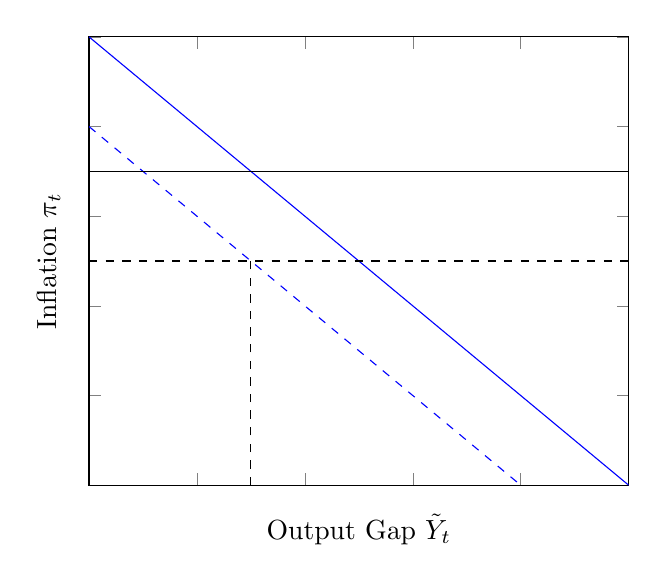
\begin{tikzpicture}
\begin{axis}[xlabel={Output Gap $\og_t$},ylabel={Inflation $\pi_t$},ymin=0,ymax=10,xmin=0,xmax=10,scale=1,yticklabels={,,},xticklabels={,,}]
\addplot[blue, domain=0:10, dashed]
{-x+8};
\addplot[blue, domain=0:10]
{-x+10};
\addplot[black, domain=0:10, dashed]
{5};
\addplot[black, domain=0:10]
{7};
\addplot[black, domain=0:10, dashed]
coordinates{(3,0) (3,5)};
\end{axis}
\end{tikzpicture}
\caption{\color{blue}AD-\color{black}SRAS Diagram}
\end{figure}

Now if at this point, the central banker stops increasing money supply (and causes $\Delta \log{M_t} = 0$) we simply go back to the original equilibrium.

Let's trace out what happens. Assuming that $\og_{-1} = 0$ and $\Delta \log{M_0} = 2$ and $=0$ for all other time periods. In other words, the central bank only does a short book.

\begin{align*}
&\pi_0 = 2 - \og_0 + 0 &\pi_0 = 0 &\implies &\og_0 = 2 \\
&\pi_1 = 0 - \og_1 + 2 &\pi_1 = 2 &\implies &\og_1 = 0 \\
&\pi_2 = 0 - \og_2 + 0 &\pi_2 = 0 &\implies &\og_2 = 0 \\
\end{align*}

Think about this for a while and you should see how we just engineered a boom in the short run.

However, if we constantly increase money supply (and cause $\Delta \log{M_t}$ to be at a constant non-zero value), then we'd just stay here at the new AD.

\begin{align*}
&\pi_0 = 2 - \og_0 + 0 &\pi_0 = 0 &\implies &\og_0 = 2 \\
&\pi_1 = 2 - \og_1 + 2 &\pi_1 = 2 &\implies &\og_1 = 2 \\
&\pi_2 = 2 - \og_2 + 2 &\pi_2 = 2 &\implies &\og_2 = 2 \\
\end{align*}

And we will persistently stay at a positive output gap.

\section{Modernizing Our Business Cycle}

Now let's just get a little more masochistic. Let's add even more things to our model.

\subsection{Positive Trend Growth}

So far, we've been assuming that the path full employment takes is flat. It's purely horizontal. That's a consequence of our medieval production function

$Y_t = \bar{A} L_t$

If we assume that there's only one full employment level $\bar{L}$, then $\bar{Y}$ will be a constant.

However, if we had $A_t$, we will achieve an increasing $\bar{Y}$.

Let's look at it from the perspective of AD and SRAS.

\[ \pi_t = \Delta \log{M_t} - \og_t + \og_{t-1} \]

\[\pi_t = \theta \og_{t-1} \]

Now with the replacement of $\bar{A}$ with $A_t$

\begin{align*}
\og_t &= \log{Y_t} - \log{\bar{Y}_t} \\
\og_t - \og_{t-1} &= \log{Y_t} - \log{\bar{Y}_t} - \log{Y_{t-1}} + \log{\bar{Y}_{t-1}} \\
&= \log{Y_t} - \log{Y_{t-1}} - \log{A_t} + \log{A_{t-1}} \\ 
\og_t - \og_{t-1} + \log{A_t} - \log{A_{t-1}} &= \log{Y_t} - \log{Y_{t-1}} \\ 
\og_t - \og_{t-1} + \Delta \log{A_t} &= \log{Y_t} - \log{Y_{t-1}}
\end{align*}

Which means that our AD becomes

\[ \pi_t  = \Delta \log{M_t} - \og_t + \og_{t-1} - \Delta \log{A_t} \]

Now this is a lot of math, but does it make intuitive sense? Well, think of the cookie factory again. If the capacity of the factory increases at a constant rate (which is what we're doing by substituting $\bar{A}$ with $A_t$) then whatever output gap we had the previous year will be affected by this growth. Say that my capacity was 100 cookies, and I was experiencing a positive output gap, so I was producing 110 cookies. This leaves me with an output gap of 10. Next year, if my capacity expands to 110 cookies, then when I'm producing 110 cookies, there's an output gap of zero.

All in all, treat $\Delta \log{A_t}$ as a constant, and realize that actual output and trend growth path both increase. It has no effect on the equations we're using for AD and SRAS and all the effects still stand.

\subsection{Okun's Law}

So far we have been talking about output gaps only. However, we want to somehow link this to unemployment. So think of \textbf{Okun's Law} as the \textbf{bridge that links output gap and unemployment.} THAT IS ALL. That is really all that Okun's Law does. 

\begin{align*}
&u_t - u^n = - \frac{1}{2} \og_t &\mathrm{or}& &\og_t = - 2(u_t - u^n)
\end{align*}

where $u_t$ is current unemployment, and $u^n$ is the \textbf{Non Accelerating Inflationary Rate of Unemployment}. In short, it is the unemployment level that will not cause crazy inflation. We'll see why that is in a while.

We can take our AD and SRAS curves and throw Okun's Law at them.

\begin{align*}
\pi_t  &= \Delta \log{M_t} - \og_t + \og_{t-1} \\
\pi_t &= \theta \og_{t-1}
\end{align*}

In the long run, we can define a certain $\bar{\og}$ that makes $\og_t - \og_{t-1} = 0$. In other words, $\bar{\og} = \og_t = \og_{t-1}$. This is our long run output gap.

Then,

\begin{align*}
\pi_t  &= \Delta \log{M_t} \\
\pi_t &= \theta \bar{\og_t}
\end{align*}

Substituting in Okun's Law

\[ \pi_t = - 2 \theta (\bar{u} - u^n) \] 

In the short run, however, we know that 

\[ \pi_t = \theta \og_{t-1} = -2 \theta (u_{t-1} - u^n) \] 

The \textbf{Phillips Curve} describes this relationship between inflation $\pi_t$ and unemployment $u_t$.

We know that in the short run, this line is horizontal line since $\pi_t = \theta \og_{t-1} = -2 \theta (u_{t-1} - u^n)$ doesn't contain the term $u_t$, hence is a horizontal line. 

However, the long run curve is downward sloping (since in the long run $\bar{u} = u_t = u_{t-1}$. 

\begin{figure}[H]
\centering
\begin{tikzpicture}
\begin{axis}[xlabel={Unemployment $u_t$},ylabel={Inflation $\pi_t$},ymin=0,ymax=10,xmin=0,xmax=10,scale=1,yticklabels={,,},xticklabels={,,}]
\addplot[blue, domain=0:10]
{-x+8};
\addplot[black, domain=0:10]
{5};
\addplot[black, domain=0:10, dashed]
coordinates{(3,0) (3,5)};
\end{axis}
\end{tikzpicture}
\caption{Phillips Curve with Short Run Phillips Curve and \color{blue} Long Run Phillips Curve}
\end{figure}

The intersection is the \textbf{NAIRU} $u^n$ since that is where $u_{t-1} = \bar{u} = u_t$

This effectively gives a trade off between inflation and unemployment. This means that the government can choose a certain level of inflation to "sacrifice" in order to get less unemployment. 

However, this doesn't actually happen in reality. What's gonna happen is that if the government sets inflation at a positive rate and achieve unemployment below $u^n$, the Phillips Curve shifts up because at each unemployment level people expect higher inflation, and will have already incorporated that into their price.

\begin{figure}[H]
\centering
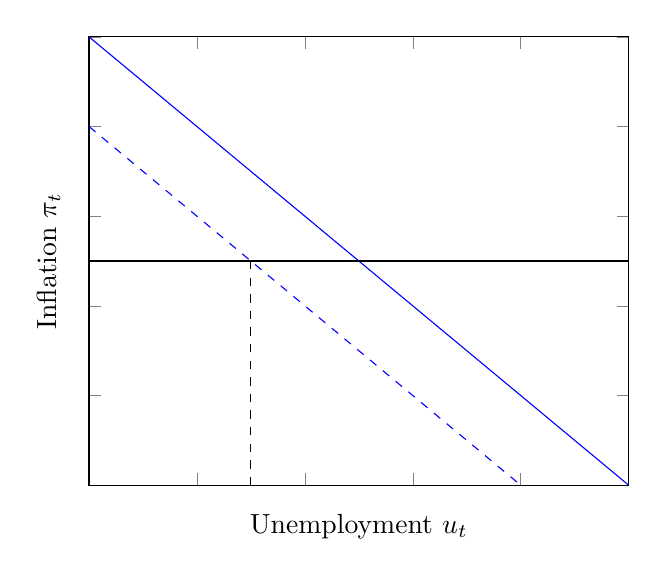
\begin{tikzpicture}
\begin{axis}[xlabel={Unemployment $u_t$},ylabel={Inflation $\pi_t$},ymin=0,ymax=10,xmin=0,xmax=10,scale=1,yticklabels={,,},xticklabels={,,}]
\addplot[blue, domain=0:10, dashed]
{-x+8};
\addplot[blue, domain=0:10]
{-x+10};
\addplot[black, domain=0:10]
{5};
\addplot[black, domain=0:10, dashed]
coordinates{(3,0) (3,5)};
\end{axis}
\end{tikzpicture}
\caption{Phillips Curve with Short Run Phillips Curve and \color{blue} Long Run Phillips Curve}
\end{figure}

To formalize this, we use the idea of expectations. We redefine inflation $\pi_t$ as 

\[ \pi_t = \mathrm{E}_{t-1} \pi_t + \bar{v} \og_t + \bar{o} \] 

Then we define $\mathrm{E}_{t-1} \pi_t = \pi_{t-1}$. In other words, people look at the past to form future expectations. 

This is \textbf{adaptive expectations}. Then this makes inflation $\pi_t$

\[ \pi_t = \pi_{t-1} + \bar{v} \og_t + \bar{o} \] 

Now we know that if $\og_t$ is positive, then the situation below happens. Assume that we start with $\og_t = 2$ and $\pi_{-1} = 0$. $\bar{v} = 1$ and $\bar{o} = 0$ for convenience.

Then,

\begin{align*}
\pi_0 &= 0 + 2 + 0 = 2 \\ 
\pi_1 &= 2 + 2 + 0 = 4 \\ 
\pi_2 &= 4 + 2 + 0 = 7
\end{align*}

In other words, so long as there is a positive $\og_t$ that persists, inflation will keep increasing. This means that the government can no longer engineer a short term boom by playing with $\Delta \log{M_t}$.

Let's apply Okun's Law and see what this does to unepmloyment.

\[ \pi_t = \pi_{t-1} - 2 \bar{v} (u_{t} - u^n) + \bar{o} \] 

Let's say that the government persistently tries to make unemployment $u_t$ below NAIRU, so $u_t - u^n = -2$. Then, using the same assumptions as earlier,

\begin{align*}
\pi_0 &= 0 - (-2) + 0 = 2 \\ 
\pi_1 &= 2 - (-2) + 0 = 4 \\ 
\pi_2 &= 4 - (-2) + 0 = 7
\end{align*}

Again, if the government sets unemployment at an artificially low level, it will incur the wrath of the inflation gods. 

Tada!

Graphically, what happens is that the Phillips Curve simply keeps shifting up if we choose an unemployment level anywhere not $u^n$. Remember, this adaptive expectation mumbo jumbo is just a formalization of the intuition that people kind of expect what's happening.







\end{document}